\documentclass[12pt]{article}
\usepackage[utf8]{inputenc}
\usepackage[T1]{fontenc}
\usepackage[a4paper]{geometry}
\geometry{hscale=0.80,vscale=0.80,centering}
\usepackage{amsmath}
\usepackage{amsthm}
\usepackage{stmaryrd}
\usepackage{amssymb}
\usepackage{breqn}
\usepackage{graphicx}
\usepackage[affil-it]{authblk}
\newcommand{\Mod}[1]{\ (\mathrm{mod}\ #1)}
\title{Projet P-A.N.D.R.O.I.D.E.\\
\bigbreak\textbf{Branch and Bound pour les diagrammes d'influence}}
\author{PINAUD David \& BIEGAS Emilie}
\date{Janvier 2021}
\affil{Université Sorbonne Sciences}
\begin{document}
\maketitle

\renewcommand{\contentsname}{Table des Matières}
\pagebreak
\tableofcontents
\pagebreak

\section{Introduction}

\subsection{Les diagrammes d'influence (ID)}
Les diagrammes d'influence (ID) sont des graphes acycliques dirigés présentant trois types de nœuds. 
Les nœuds \textit{chances}, illustrés graphiquement par un ovale, représentent des variables aléatoire (dont le domaine est fini et non vide). 
Les nœuds de \textit{décision}, illustrés graphiquement par un rectangle, représentent des variables de décision (dont le domaine est fini et non vide) tandis que les nœuds \textit{utilitaire}, illustrés graphiquement par un losange, représentent une fonction d'utilité locale exprimant la préférence.
Les arêtes de ce graphe représentent une dépendance entre les nœuds et ont une signification différente en fonction du type de nœud à son extrémité.
En effet, si une arête pointe vers un nœud aléatoire, cela représente une dépendance probabiliste; si elle pointe vers un nœud de décision, elle a un but informatif; enfin, si elle pointe vers un nœud utilitaire, elle représente une dépendance fonctionnelle.
\bigbreak
Les IDs respectent deux hypothèses, une hypothèse de régularité (les décisions sont ordonnées dans le temps) et une hypothèse dite non-oubliant (chaque décision est conditionnée par toutes les observations de décisions antérieures).
L'ensemble des instanciations des noeuds chances pour les décisions antérieurs d'une certain désicion est appelé l'\textit{historique}.


\subsection{Les LIMIDs}
 Les \textit{LImited-Memory Influence-Diagrams} (LIMIDs) sont des diagrammes d'influence qui assouplissent les deux hypothèses précédemment citées. Tout d'abord, les LIMIDs assouplissent l'hypothèse non-oubliant de manière à conditionner une décision sur un nombre limité d'observations et de décisions antérieurs pertinentes (pour un compromis qualité/complexité).
Ensuite, assouplir l'hypothèse de régularité permet par exemple de modéliser la coopération de problèmes de décision multi-agents où un agent n'est pas au courant de décision d'autres agents. On peut aussi facilement transformer un ID en LIMID.

\subsection{Limites des implémentations actuelles}
Les méthodes de résolution exactes actuelles de LIMIDs ou IDs sont limités par leur complexité en temps et en espace.
Pour exemple, considérons un ID qui modélise un robot dans un labyrinthe représenté par une matrice $n\times m$ composé de cases \textit{mur}, de cases \textit{libre} et d'une case \textit{objectif}. On représente le labyrinthe comme ci-dessous, les cases grises, blanches, et étoilés étant respectivement les cases \textit{mur}, \textit{libre}, et \textit{objectif}.
\begin{figure}[b]
\centering
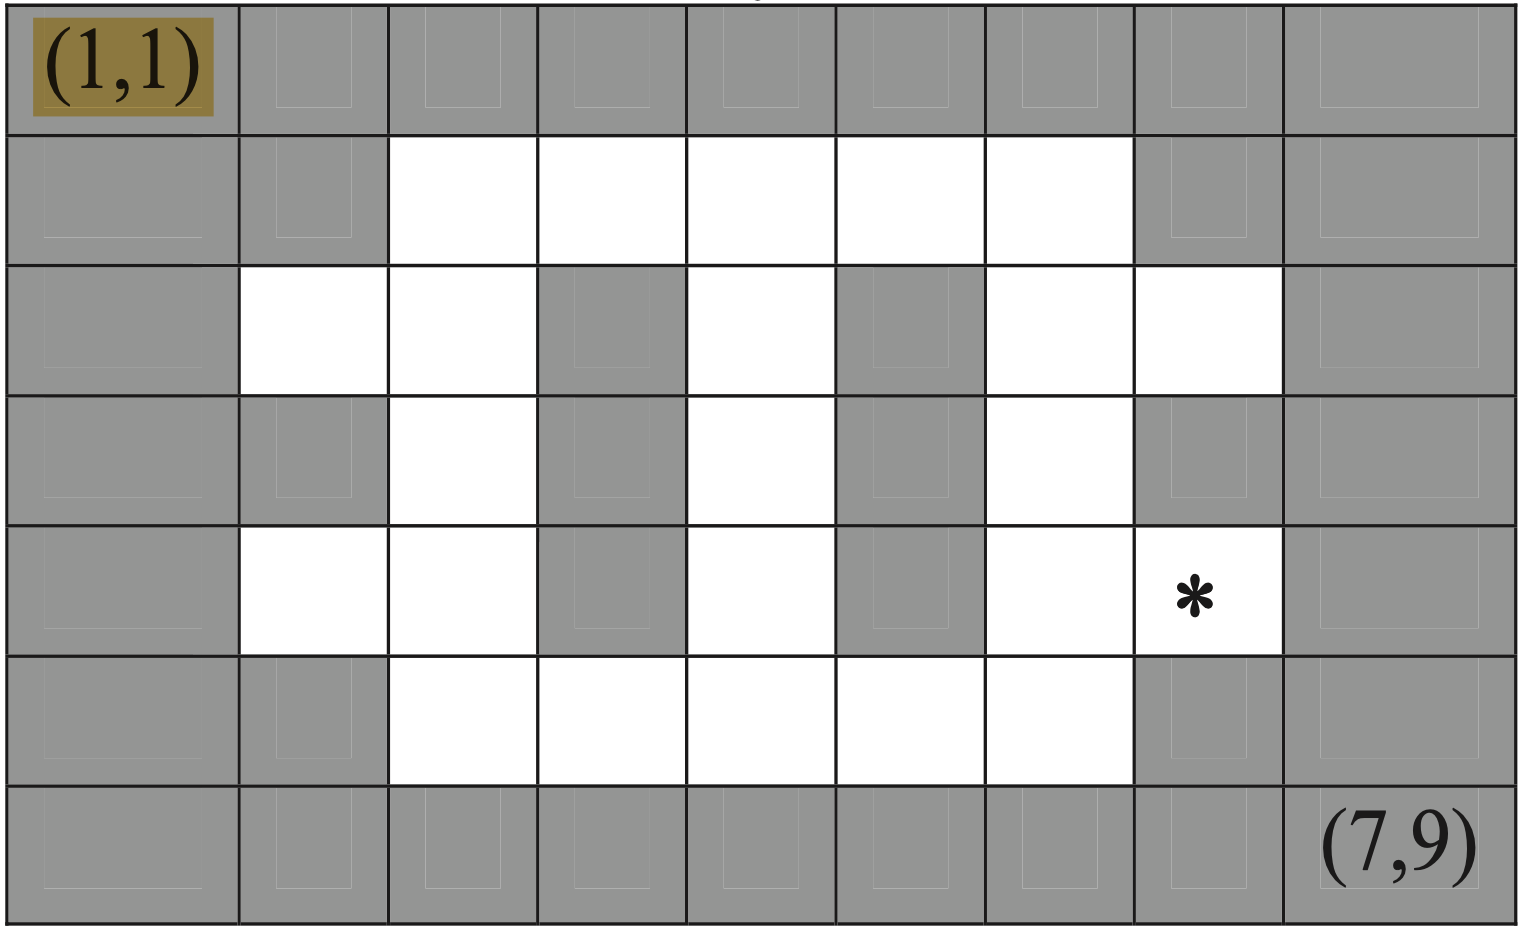
\includegraphics[scale=0.2]{docs/MAZE.png}
\caption{Un exemple de représentation d'un labyrinthe $9\times 7$}
\end{figure}
\pagebreak


Le robot est initialement placé sur une des cases \textit{libre} et l'objectif du robot est d'atteindre la case \textit{objectif}. 
À chaque étape, le robot peut se déplacer dans toutes les directions (nord, sud, est, ouest et les diagonales) d'une seule case ou choisir de ne pas se déplacer. Il possède quatre capteurs pointés vers les quatre cardinaux qui indiquent au robot la présence d'un mur ou non.
%les probabilités sommes à 1 --> c'est bien une distribution donc pas de mouvement en diagonale possible ?!

À chaque étape, le robot choisit une direction cardinale où faire un pas puis le mouvement du robot suit une mesure de probabilité :
\begin{itemize}
  \item Un pas vers la case voulu a une probabilité $pBouger$ de réussir.
  \item Échouer de bouger survient avec probabilité $pEchecBouger$.
  \item À chaque étape, il y a une chance que le robot fasse un mouvement erratique:
  \begin{itemize}
        \item Faire un pas vers l'est ou vers l'ouest (s'il est possible de le faire) survient avec une probabilité de $pCote$ dans chacun des deux cas.
        \item Faire un pas vers le sud (s'il est possible de le faire) survient avec une probabilité $pArriere$.
        \end{itemize}
  \item Un pas vers un \textit{mur} a une probabilité de 0.
  \item Les autres probabilités sont normalisées afin de former une distribution de probabilité.
\end{itemize}
\begin{figure}[h]
\centering
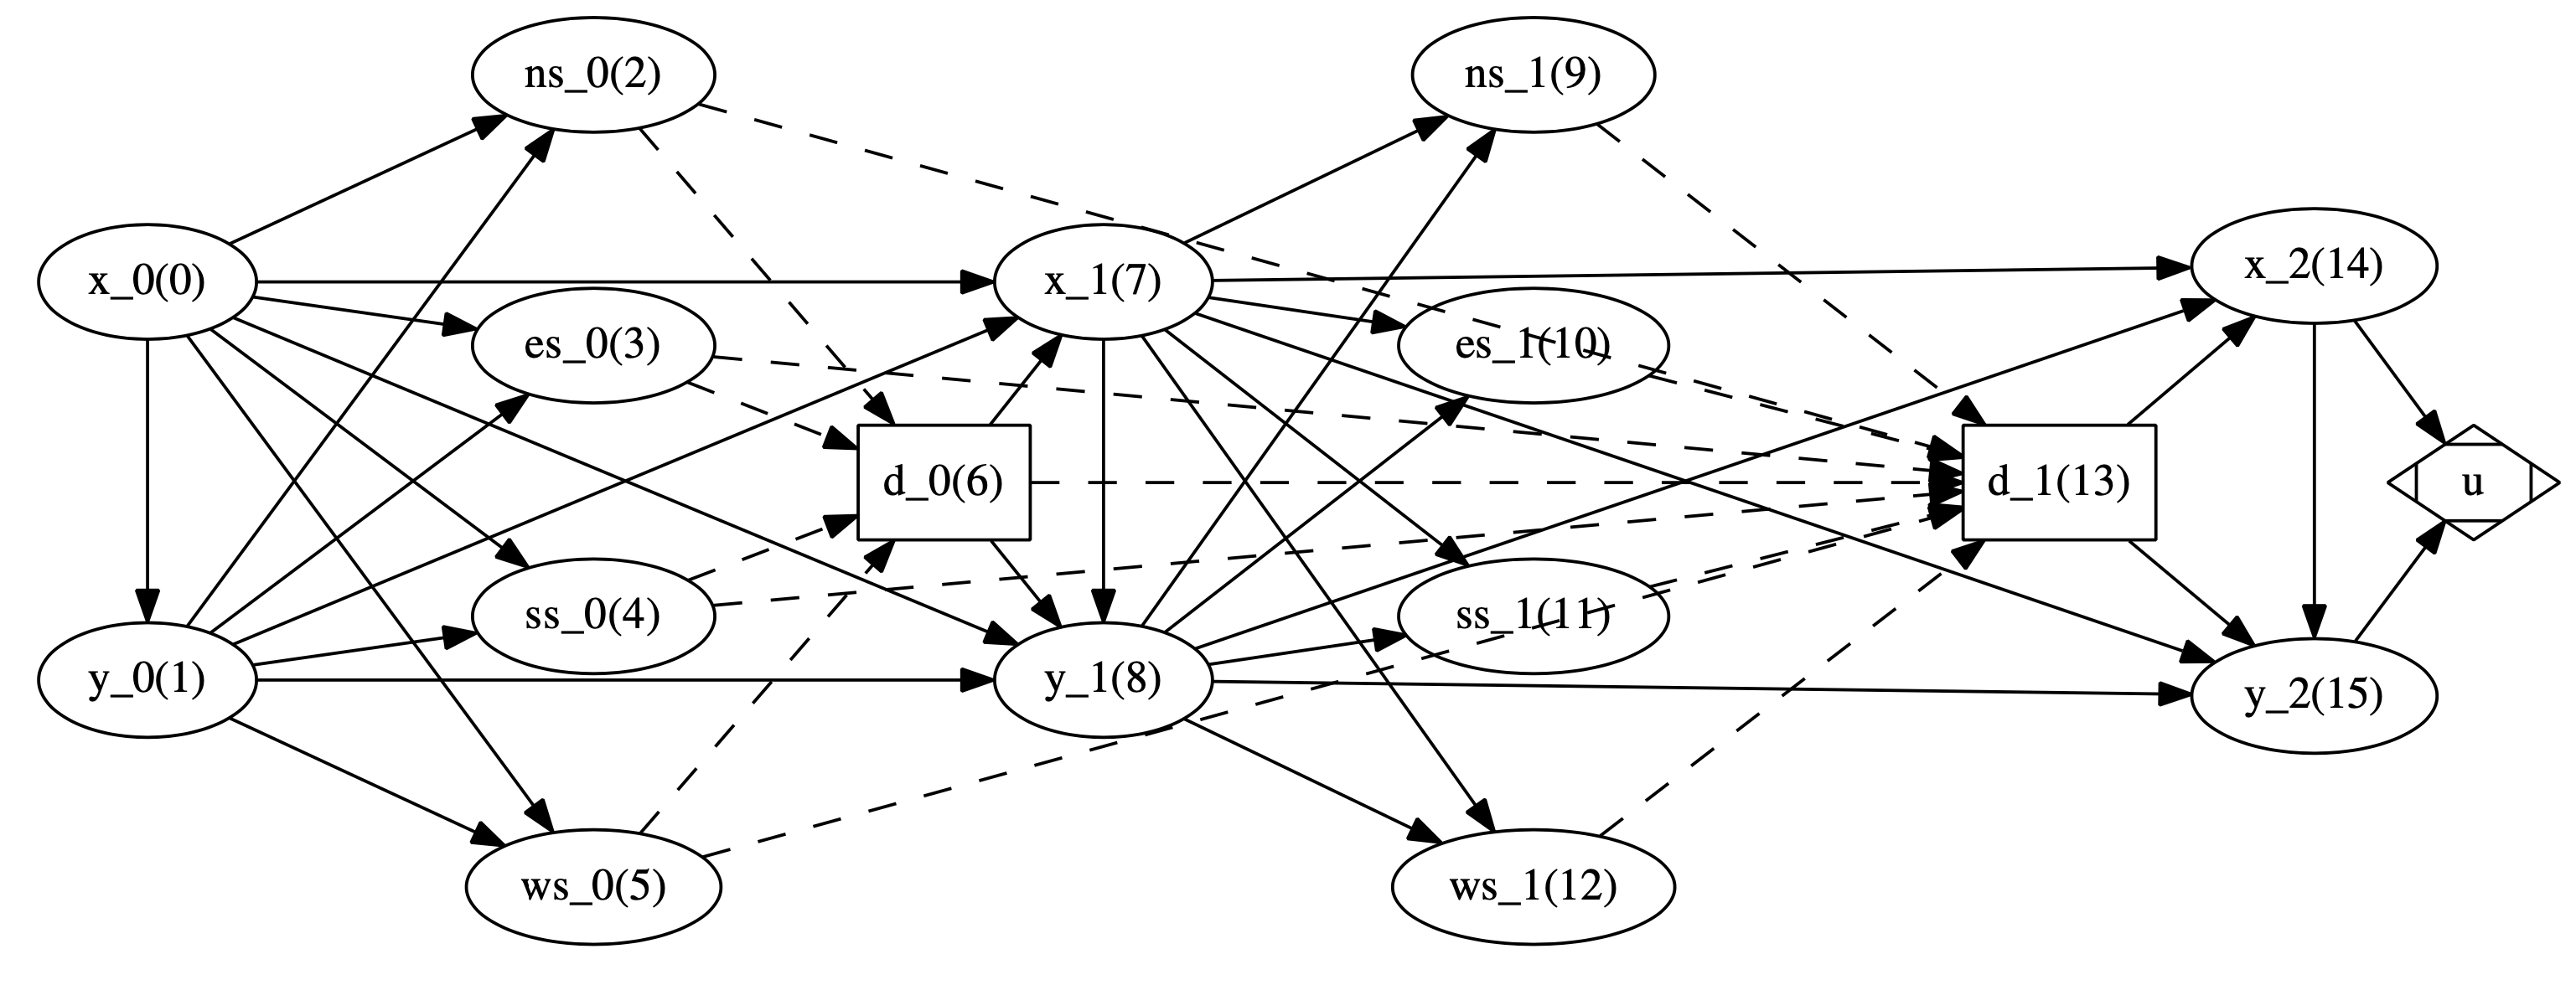
\includegraphics[scale=0.32]{docs/IDROBOT.png}
\caption{L'ID modélisant le problème du robot à deux étapes }
\end{figure}
A l'étape $i$, les noeuds chances $x_i$ et $y_i$ représentent les coordonnées du robot sur la grille, $ns_i, es_i, ss_i, ws_i$ les capteurs du robot dans les sens nord, est, sud et ouest respectivement. Les noeuds $d_i$ sont les noeuds de décisions.

\pagebreak
Pour visualiser le caractère exponentiel de la complexité en espace, voici un tableau récapitulatif des tailles des arbres de jonctions selon le nombre d'étapes ainsi que les graphes associés.
\bigbreak
\bigbreak
   \begin{tabular}{|p{3cm} || p{3cm} | p{3cm} | p{3cm} | p{3cm} | }
    \hline
    Nombre d'étapes & temps pour l'inférence & temps pour l'arbre de jonction & largeur de l'arbre & taille en mémoire de l'arbre (en Go) \\ 
    \hline
    2&0.077&0.000&11&2 E-3\\
    \hline
    3&0.083&0.010&15&38 E-3\\
    \hline
    4&0.104&0.010&20&787 E-3\\
    \hline
    5&0.140&0.011&24&12\\
    \hline
    6&0.264&0.017&29&984\\
    \hline
    7&0.178&0.011&34&76 E3\\
    \hline
    8&0.254&0.016&37&246 E3\\
    \hline
    9&0.330&0.014&42&19687 E3\\
    \hline
    10&0.398&0.019&46&315000 E3\\
    \hline
   \end{tabular}
 \begin{figure}[h]
\centering
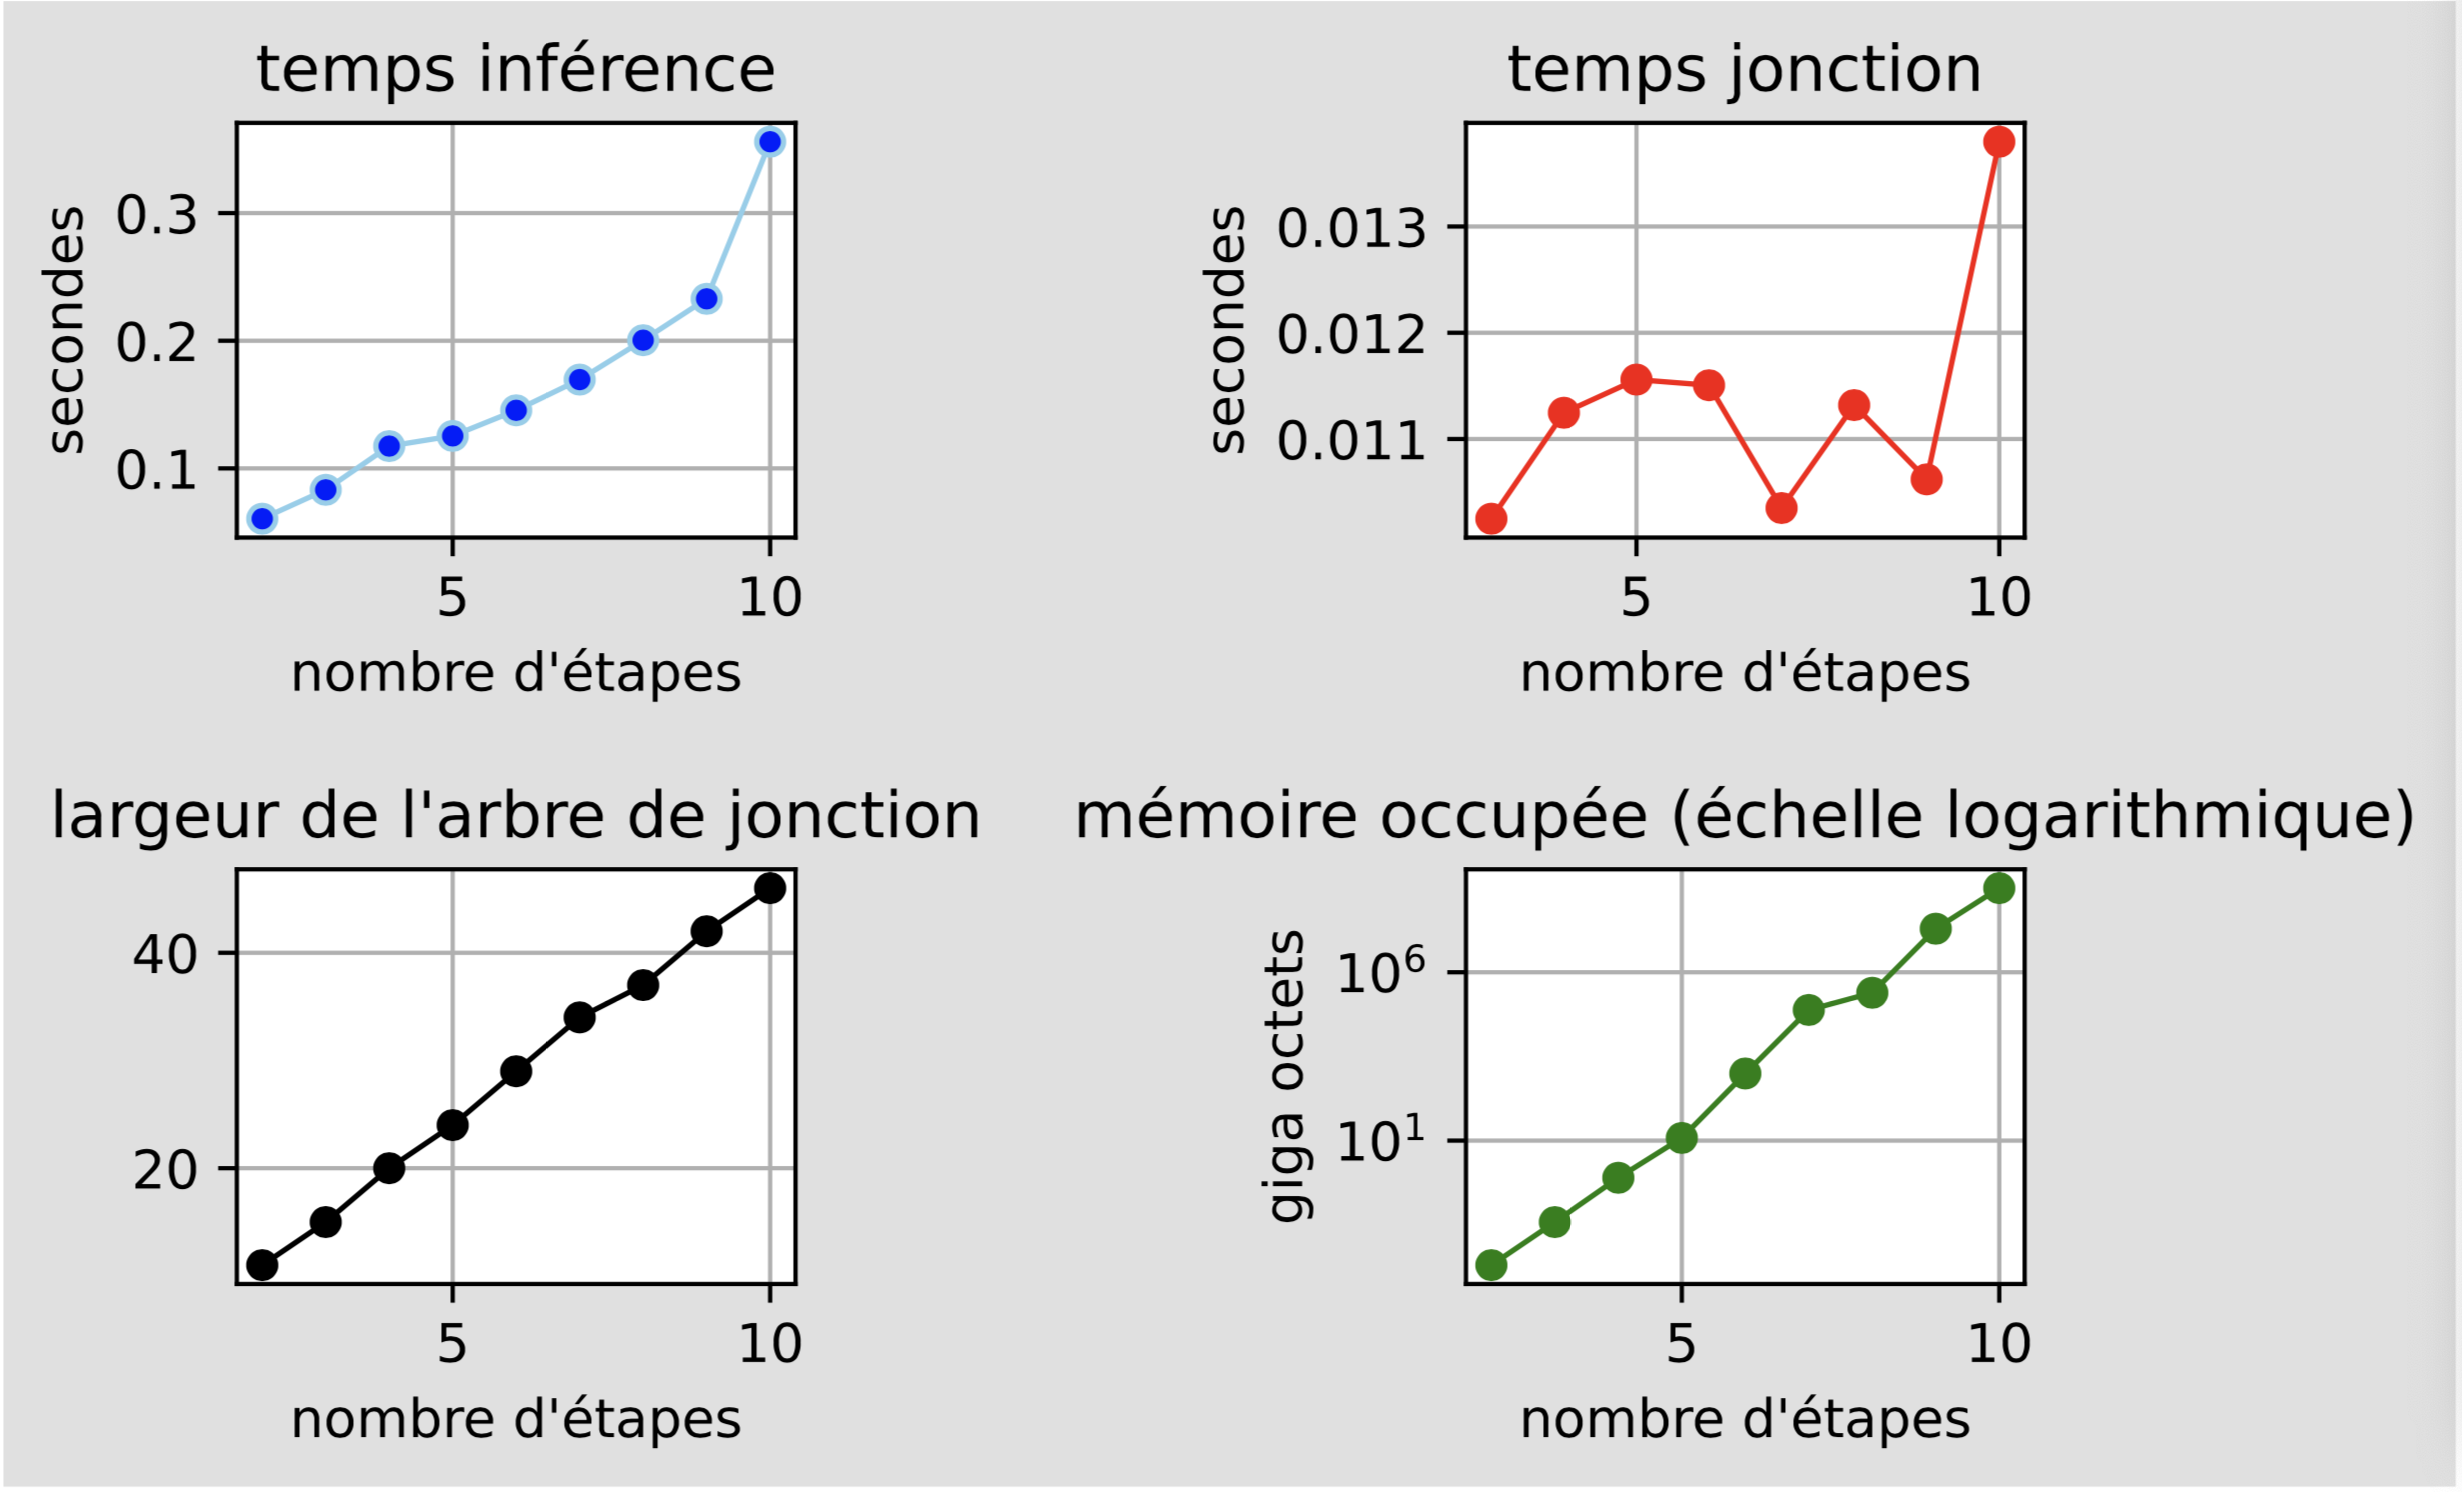
\includegraphics[scale=0.32]{docs/graphes.png}
\caption{Graphes sur la complexité en temps et espace des méthodes actuelles}
\end{figure}
\bigbreak
\bigbreak
On parvient à résoudre cet ID avec les méthodes exactes actuelles (une machine avec 128Go de mémoire vive) sur des instances du problèmes comprenant jusqu'à 5 étapes. Au delà de 5 étapes, la mémoire nécessaire et le temps pour trouver la solution explose. Il n'est pas envisageable de concevoir une machine capable de stocker autant de données pour résoudre de façon exacte cet ID. Il y a donc un réel besoin d'avoir une implémentation permettant de résoudre plus rapidement les ID et en nécessitant moins d'espace.

\subsection{But du projet}
Le but de ce projet est alors d'implémenter en utilisant un algorithme heuristique basé sur le Branch and Bound pour résoudre ce type de problème à complexité en espace et en temps très grande. %Pour ce faire, nous allons nous baser sur une étude menée en 2013
%Pour ce faire, on doit tirer parti des opportunités pour le calcul de stratégie, utiliser des techniques d'inférence probabiliste et calculer les limites dans un graphe.
[...]
Le but final de ce projet est l'intégration de notre algorithme dans la librairie Python PyAgrum. Pour cela, il faut que notre code soit compatible avec les inférences existantes, avec les notebooks ...



\end{document}